\documentclass[12pt, a4paper]{report}

 % --- Pacchetti fondamentali ---
\usepackage[utf8]{inputenc}
\usepackage[T1]{fontenc}
\usepackage[italian]{babel}
\usepackage{geometry}
\geometry{a4paper, top=2.5cm, bottom=2.5cm, left=2.5cm, right=2.5cm}
\usepackage{graphicx}
\usepackage[numbers, square]{natbib}
\usepackage[hidelinks]{hyperref}
\usepackage{cleveref} % deve venire dopo hyperref
\usepackage{float}
\usepackage{xcolor}
\usepackage{parskip}
\usepackage[font=small,labelfont=bf]{caption}
\usepackage{subcaption}
\usepackage{microtype} 
\usepackage{lmodern}

\usepackage{booktabs}

% --- Listings (Configurazione JSON) ---
\usepackage{listings}
\definecolor{codegreen}{rgb}{0,0.6,0}
\definecolor{codegray}{rgb}{0.5,0.5,0.5}
\definecolor{codepurple}{rgb}{0.58,0,0.82}
\definecolor{backcolour}{rgb}{0.95,0.95,0.92}
\definecolor{punct}{RGB}{100,100,100}
\definecolor{numb}{RGB}{0,102,204}
\definecolor{delim}{RGB}{20,105,176}
\definecolor{json_key}{RGB}{18, 110, 213}    % Blu per le chiavi
\definecolor{json_string}{RGB}{0, 153, 51}  % Verde per i valori stringa
\definecolor{json_number}{RGB}{255, 102, 0} % Arancione per i numeri

\lstdefinelanguage{json}{
    basicstyle=\ttfamily\footnotesize,
    numbers=left,
    numberstyle=\tiny\color{codegray},
    stepnumber=1,
    numbersep=8pt,
    showstringspaces=false,
    breaklines=true,
    frame=lines,
    stringstyle=\color{json_string},
    morestring=[b]",
    backgroundcolor=\color{backcolour},
    moredelim=[is][\color{json_key}]{||}{||},
    literate=
     *{0}{{{\color{json_number}0}}}{1}
      {1}{{{\color{json_number}1}}}{1}
      {2}{{{\color{json_number}2}}}{1}
      {3}{{{\color{json_number}3}}}{1}
      {4}{{{\color{json_number}4}}}{1}
      {5}{{{\color{json_number}5}}}{1}
      {6}{{{\color{json_number}6}}}{1}
      {7}{{{\color{json_number}7}}}{1}
      {8}{{{\color{json_number}8}}}{1}
      {9}{{{\color{json_number}9}}}{1}
      {:}{{{\color{punct}{:}}}}{1}
      {,}{{{\color{punct}{,}}}}{1}
      {\{}{{{\color{delim}{\{}}}}{1}
      {\}}{{{\color{delim}{\}}}}}{1}
      {[}{{{\color{delim}{[}}}}{1}
      {]}{{{\color{delim}{]}}}}{1}
}


\hypersetup{
    pdftitle={BuySellChain - Documento di Progettazione e Analisi di Sicurezza},
    pdfauthor={Salvucci Franco, Ionut Georgian Zbirciog},
    pdfsubject={Sistema d'Asta Trustless su Hyperledger Fabric},
    pdfkeywords={Blockchain, Hyperledger Fabric, Asta, Smart Contract}
}

% Ambiente "Definizione" migliorato
\newenvironment{definizione}[1][]{
    \vspace{10pt}\par\noindent\textbf{Definizione%
    \if\relax\detokenize{#1}\relax\else\ (\textit{#1})\fi.}\itshape\ }{\vspace{10pt}\par}

% --- Dati del documento ---
\title{
    \vspace{2cm}
    {\Huge\bfseries BuySellChain}\\
    \vspace{0.5cm}
    {\Large Sistema d'Asta Trustless su Blockchain Hyperledger Fabric}\\
    \vspace{1cm}
    {\small Documento di Progettazione e Analisi di Sicurezza }
}

\author{
    \textbf{Salvucci Franco} (Mat. 0368692) \\
    \textbf{Ionut Georgian Zbirciog} (Mat. 0381279)
}
\date{27 gennaio 2026}

\begin{document}

\maketitle

% Sommario (Abstract per report)
\cleardoublepage
\begin{abstract}
    Il mercato immobiliare tradizionale è caratterizzato da inefficienze e dipendenza da intermediari. 
    \texttt{BuySellChain} propone un sistema decentralizzato basato su \textbf{Blockchain} per eliminare l'agente immobiliare fisico. 
    L'architettura su Hyperledger Fabric gestisce tramite Smart Contract la validazione delle offerte e il trasferimento della proprietà digitale. 
    Il sistema garantisce trasparenza assoluta e azzeramento delle commissioni.
\end{abstract}

\cleardoublepage
\tableofcontents

\cleardoublepage
% Assicurati che questi file esistano o usa il testo direttamente qui
\chapter{Introduzione}

Il sistema \texttt{BuySellChain} mira a decentralizzare il mercato immobiliare tramite un servizio di aste online. Come verrà illustrato, l'agente si limita alla registrazione dell'asta e non svolge più il ruolo di intermediario tipico del modello tradizionale. In questa architettura, l'intermediazione è affidata alla Blockchain, incaricata di validare ogni offerta. Questo approccio garantisce trasparenza, sicurezza e una riduzione dei costi operativi, eliminando la necessità di intermediari tradizionali e consentendo agli utenti di partecipare direttamente al processo di compravendita.

La documentazione di questo progetto è organizzata come segue:

\begin{description}
    \item[Architettura del Sistema] Saranno presentate l'architettura e le tecnologie utilizzate, con particolare attenzione al backend e alla Blockchain.
    \item[Analisi del Perimetro di Attacco] Verranno delineati il perimetro di attacco e le principali minacce.
    \item[Possibili Attacchi e Come Difendersi] Infine, saranno discussi i possibili attacchi e le contromisure adottate per mitigarli.
\end{description}

\chapter{Architettura del Sistema}

L'architettura di \textbf{BuySellChain} adotta un approccio ibrido che integra la flessibilità del Web 2.0 con la sicurezza del Web 3.0. Il sistema è progettato per garantire la disintermediazione della compravendita immobiliare, come richiesto dagli obiettivi di progetto.

\begin{description}
    \item[Frontend:] Interfaccia utente realizzata con \textbf{Jinja2} e \textbf{Alpine.js}, che fornisce reattività lato client senza richiedere una build pipeline complessa. La responsabilità è limitata alla presentazione dei dati e all'interazione utente, senza contenere logica di business critica.
    
    \item[Backend (Security Gateway):] 
    Server applicativo implementato in \textbf{Python} con il microframework \textbf{Flask}, che funge da middleware di sicurezza tra il client pubblico e la rete privata Blockchain. Questa componente ha il ruolo critico di sanitizzare gli input, gestire le sessioni, implementare il controllo degli accessi basato su ruoli (RBAC) e prevenire l'esposizione diretta delle API del Ledger. Si occupa dell'autenticazione degli utenti tramite credenziali verificate sul database off-chain e della generazione di JWT per l'autorizzazione stateless delle operazioni successive.
    
    \item[Blockchain Layer:] 
    Il nucleo del sistema, basato su \textbf{Hyperledger Fabric} \cite{HyperledgerFabricDocs}, che funziona come database distribuito e immutabile per le operazioni critiche di compravendita. Questo livello è accessibile esclusivamente tramite il client Lisp fornito dal docente, che incapsula la logica di interazione con il chaincode e la gestione delle identità crittografiche (MSP). Il meccanismo di consenso distribuito valida le transazioni secondo le regole definite negli Smart Contract, garantendo l'integrità e la non-ripudiabilità delle operazioni.
    
    \item[Database Off-Chain:] 
    Un database relazionale \textbf{PostgreSQL} utilizzato per la persistenza dei dati sensibili e non critici per il consenso distribuito, come i profili utente, le credenziali di accesso al portale web e l'anagrafe del sistema. L'accesso è mediato attraverso \textbf{SQLAlchemy}, un'astrazione ORM che garantisce protezione contro attacchi SQL injection. Questa separazione garantisce la conformità alle normative sulla privacy (GDPR), evitando la scrittura di dati sensibili sul Ledger immutabile. Le password sono protette mediante l'algoritmo di hashing bcrypt con salt unico per ogni utente.
\end{description}

\begin{figure}[H]
    \centering
    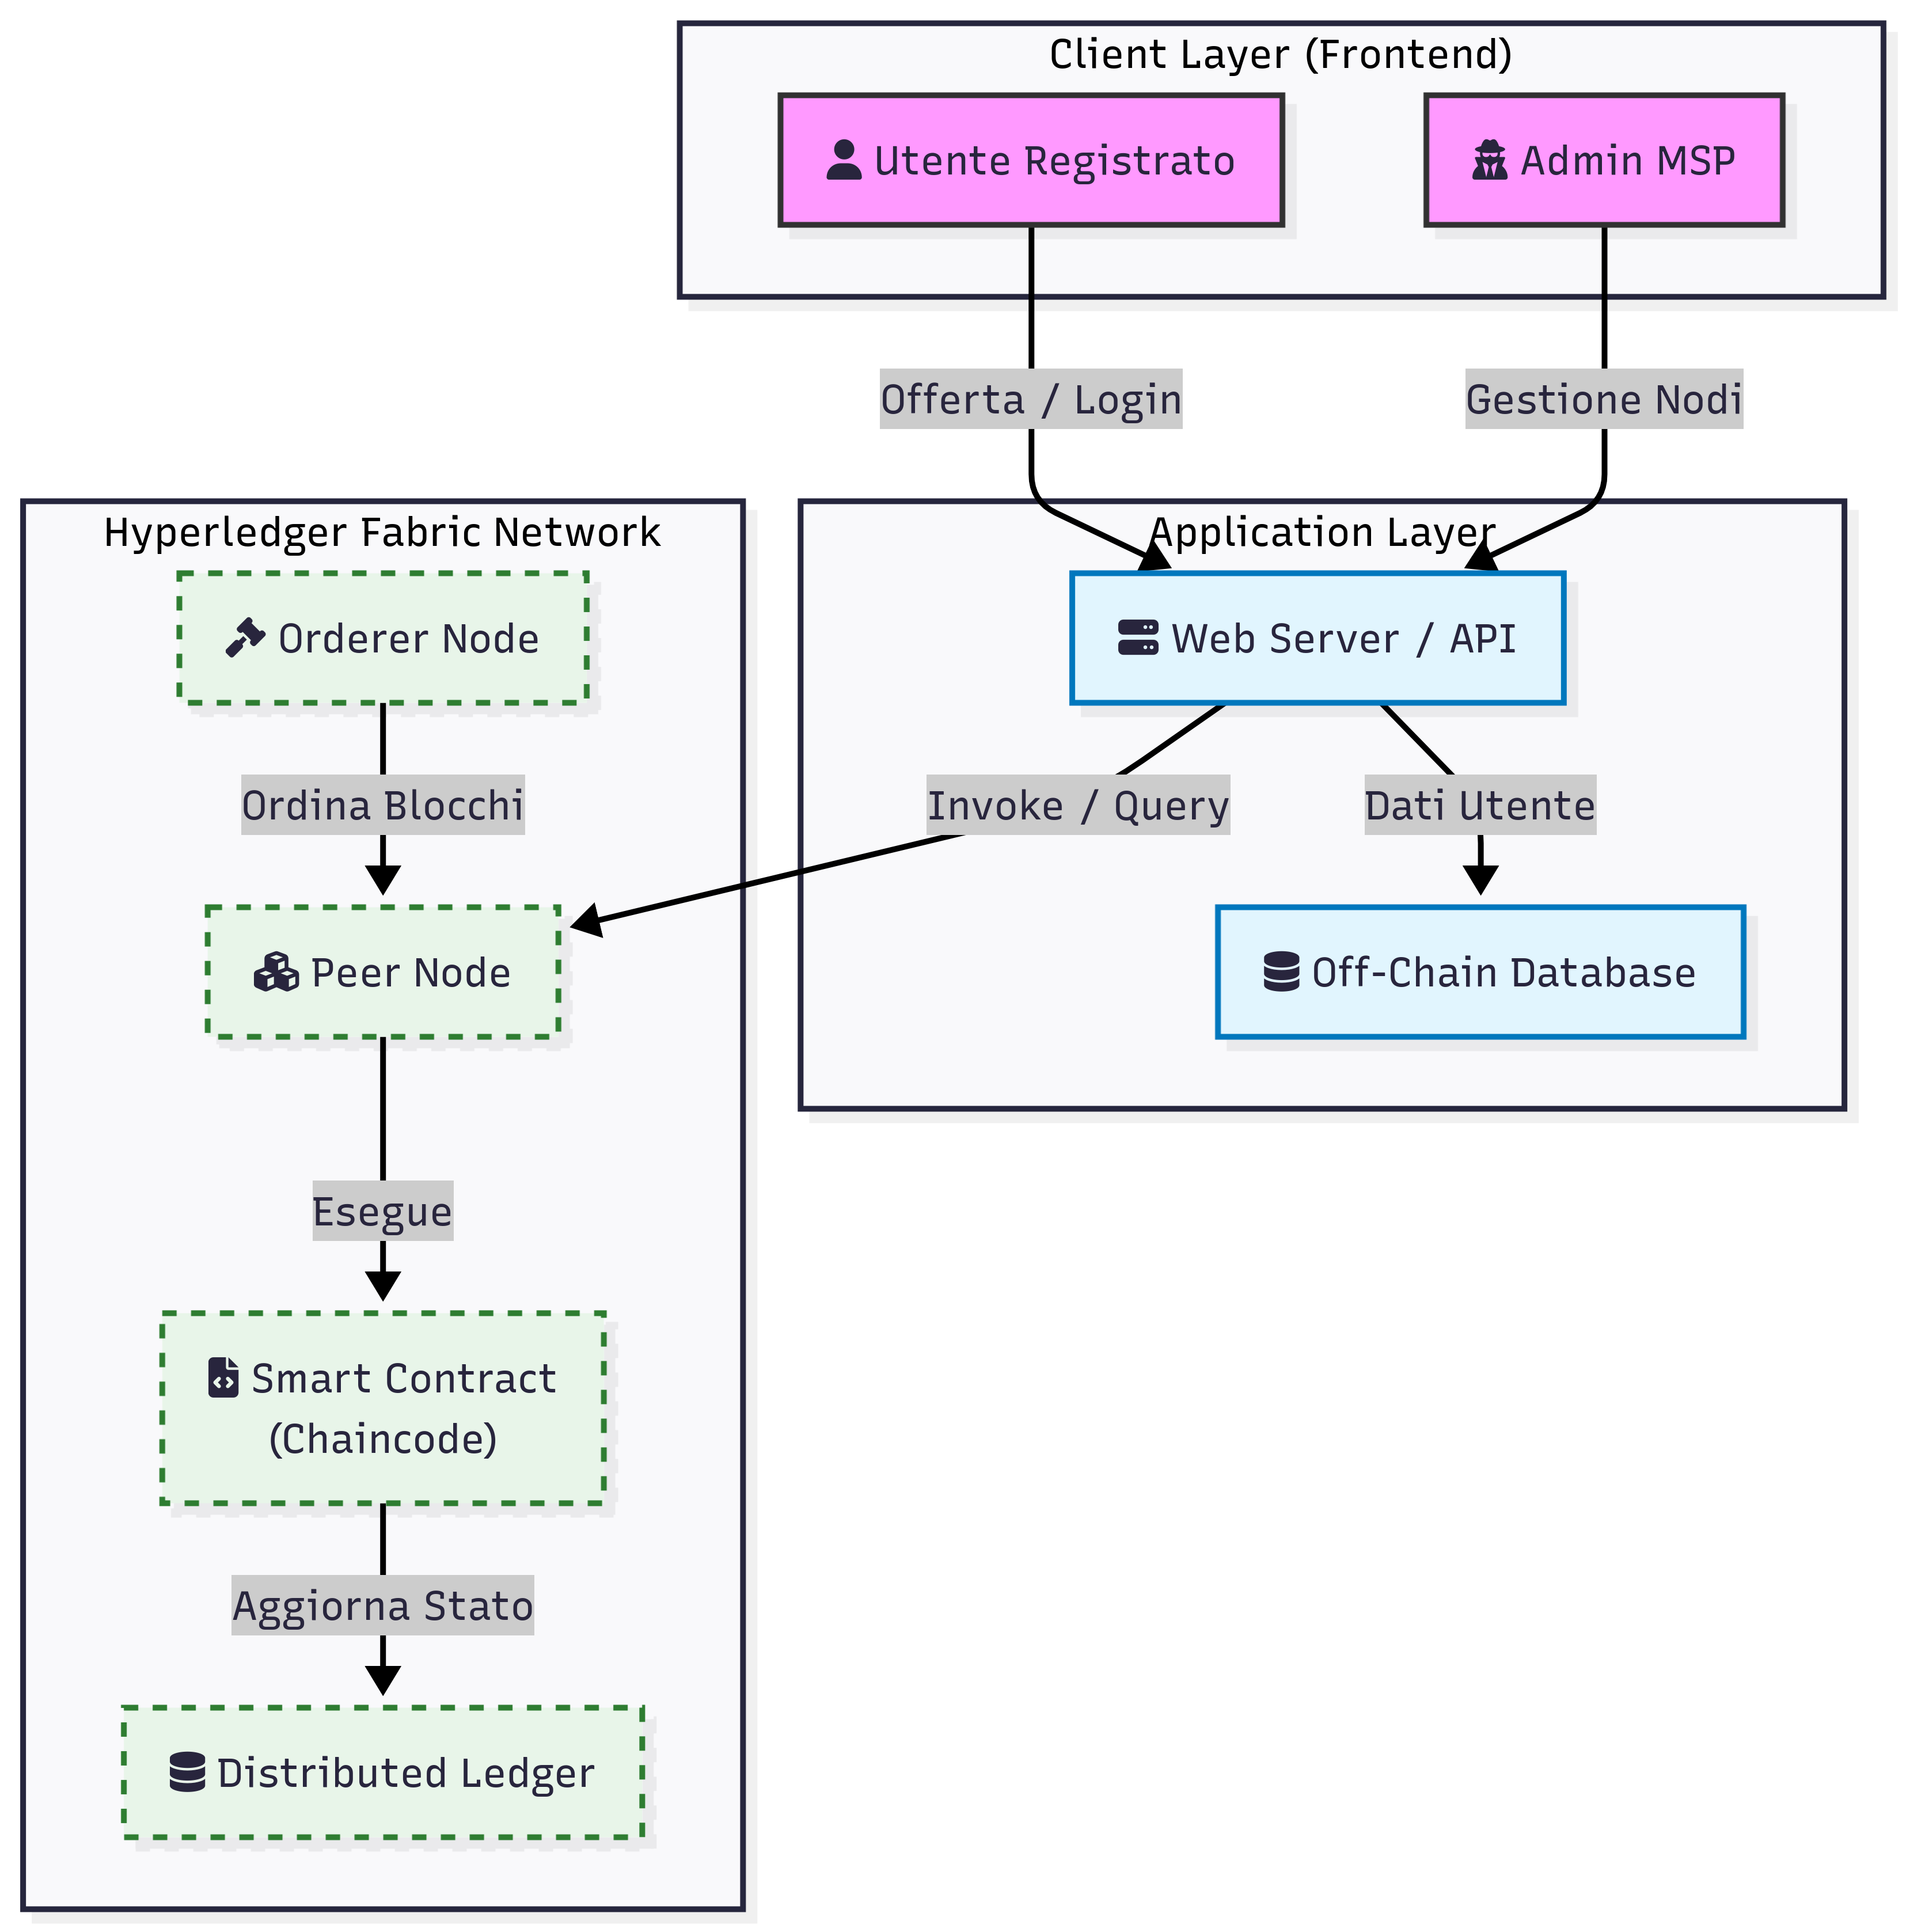
\includegraphics[width=0.6\textwidth]{images/network_arch.png}
    \caption{Schema ad alto livello dell'architettura ibrida Web 2.0 / Web 3.0}
    \label{fig:architettura}
\end{figure}

\section{Gestione dell'Identità e Sicurezza}

Poiché Hyperledger Fabric è una rete di tipo \textit{permissioned}, a differenza delle blockchain pubbliche, tutti i partecipanti devono essere identificati e autorizzati prima di poter interagire con il ledger. In questo contesto, la fiducia non è anonima ma basata su identità crittografiche verificate.

Per gestire questo livello di autorizzazione, l'architettura si basa su un componente fondamentale:

\begin{definizione}[Membership Service Provider (MSP)]
L'MSP è il componente astratto del sistema che definisce le regole di validazione delle identità. Esso agisce come un'autorità di certificazione logica che consente alla rete di riconoscere e considerare affidabili i certificati digitali presentati dai peer e dagli utenti.
\end{definizione}

\noindent Il funzionamento operativo coinvolge la cooperazione tra MSP e le \textit{Certificate Authorities} (CA):
\begin{enumerate}
    \item \textbf{Rilascio dell'Identità:} Le CA generano una coppia di chiavi (pubblica e privata) e rilasciano un certificato X.509 che rappresenta l'identità digitale dell'attore.
    \item \textbf{Verifica (Ruolo dell'MSP):} Quando un attore (es. un Peer) firma digitalmente una transazione usando la propria chiave privata, l'MSP interviene per verificare che tale certificato sia stato emesso da una CA fidata e che l'attore possieda i permessi necessari per quella specifica operazione (es. avallare una transazione).
\end{enumerate}
In questo scenario, il client Lisp incapsula tale processo; di conseguenza l'attenzione è rivolta all'autenticazione dell'utente presso il server Web (Security Gateway).

\section{User Requirements Definition}
In questa sezione vengono definiti gli attori che interagiscono con la piattaforma \textbf{BuySellChain} e le azioni a loro consentite. Il sistema è progettato per operare in un ambiente \emph{trustless} basato su Hyperledger Fabric, eliminando la necessità di intermediari umani nella fase di negoziazione.

\subsection*{User Classes and Characteristics}
\begin{description}
    \item[Amministratore di Sistema:]
    Gestisce la piattaforma, monitora anomalie e alert di sicurezza. Dispone di una dashboard dedicata per osservabilità, auditing e interventi correttivi.
    
    \item[Utente Registrato:]
    Attore abilitato alla compravendita; lo stesso account può ricoprire ruoli distinti:
    \begin{itemize}
        \item \textbf{Venditore (Proprietario dell'asset):} Possiede l'immobile digitalizzato sul registro e avvia l'asta definendone i parametri.
        \item \textbf{Offerente (Bidder):} Partecipa all'asta inviando offerte firmate e vincolanti secondo le regole dello Smart Contract.
    \end{itemize}
    
    \item[Utente Non Autenticato:]
    Visitatore esterno. Senza account può consultare le aste e gli immobili pubblicati, senza possibilità di interazione avanzata.
\end{description}

\subsection*{User Actions and Use Cases}
Le azioni riflettono la logica di business gestita dal server Web e dagli Smart Contract.

\begin{itemize}
    \item \textbf{Azioni Utente Non Autenticato:}
    \begin{itemize}
        \item Consultare la landing page del progetto.
        \item Registrarsi o accedere.
        \item Effettuare un login sicuro.
    \end{itemize}

    \item \textbf{Azioni dell'Amministratore (Monitoraggio e Sicurezza):}
    \begin{itemize}
        \item Monitorare gli alert su tentativi di violazione dell'integrità (mismatch crittografici).
        \item Analizzare i log delle offerte rifiutate per violazioni delle finestre temporali (anti-frontrunning).
    \end{itemize}
    
    \item \textbf{Azioni dell'Utente Registrato — Venditore:}
    \begin{itemize}
        \item Avviare un'asta per un immobile già digitalizzato.
        \item Impostare la finestra temporale dell'asta (inizio/fine) gestita dallo Smart Contract.
        \item Visualizzare in tempo reale sul Ledger lo stato delle offerte ricevute.
        \item Ricevere la notifica di aggiudicazione e il trasferimento della proprietà digitale.
    \end{itemize}

    \item \textbf{Azioni dell'Utente Registrato — Offerente:}
    \begin{itemize}
        \item Consultare le aste immobiliari attive.
        \item Inviare un'offerta firmata; lo Smart Contract verifica l'incremento minimo richiesto.
        \item Verificare la propria posizione in graduatoria (anonimizzata o pubblica secondo la logica di business).
        \item Visualizzare l'esito della validazione (accettata/rifiutata per motivi temporali o di importo).
    \end{itemize}
\end{itemize}

\begin{figure}[h!]
    \centering
    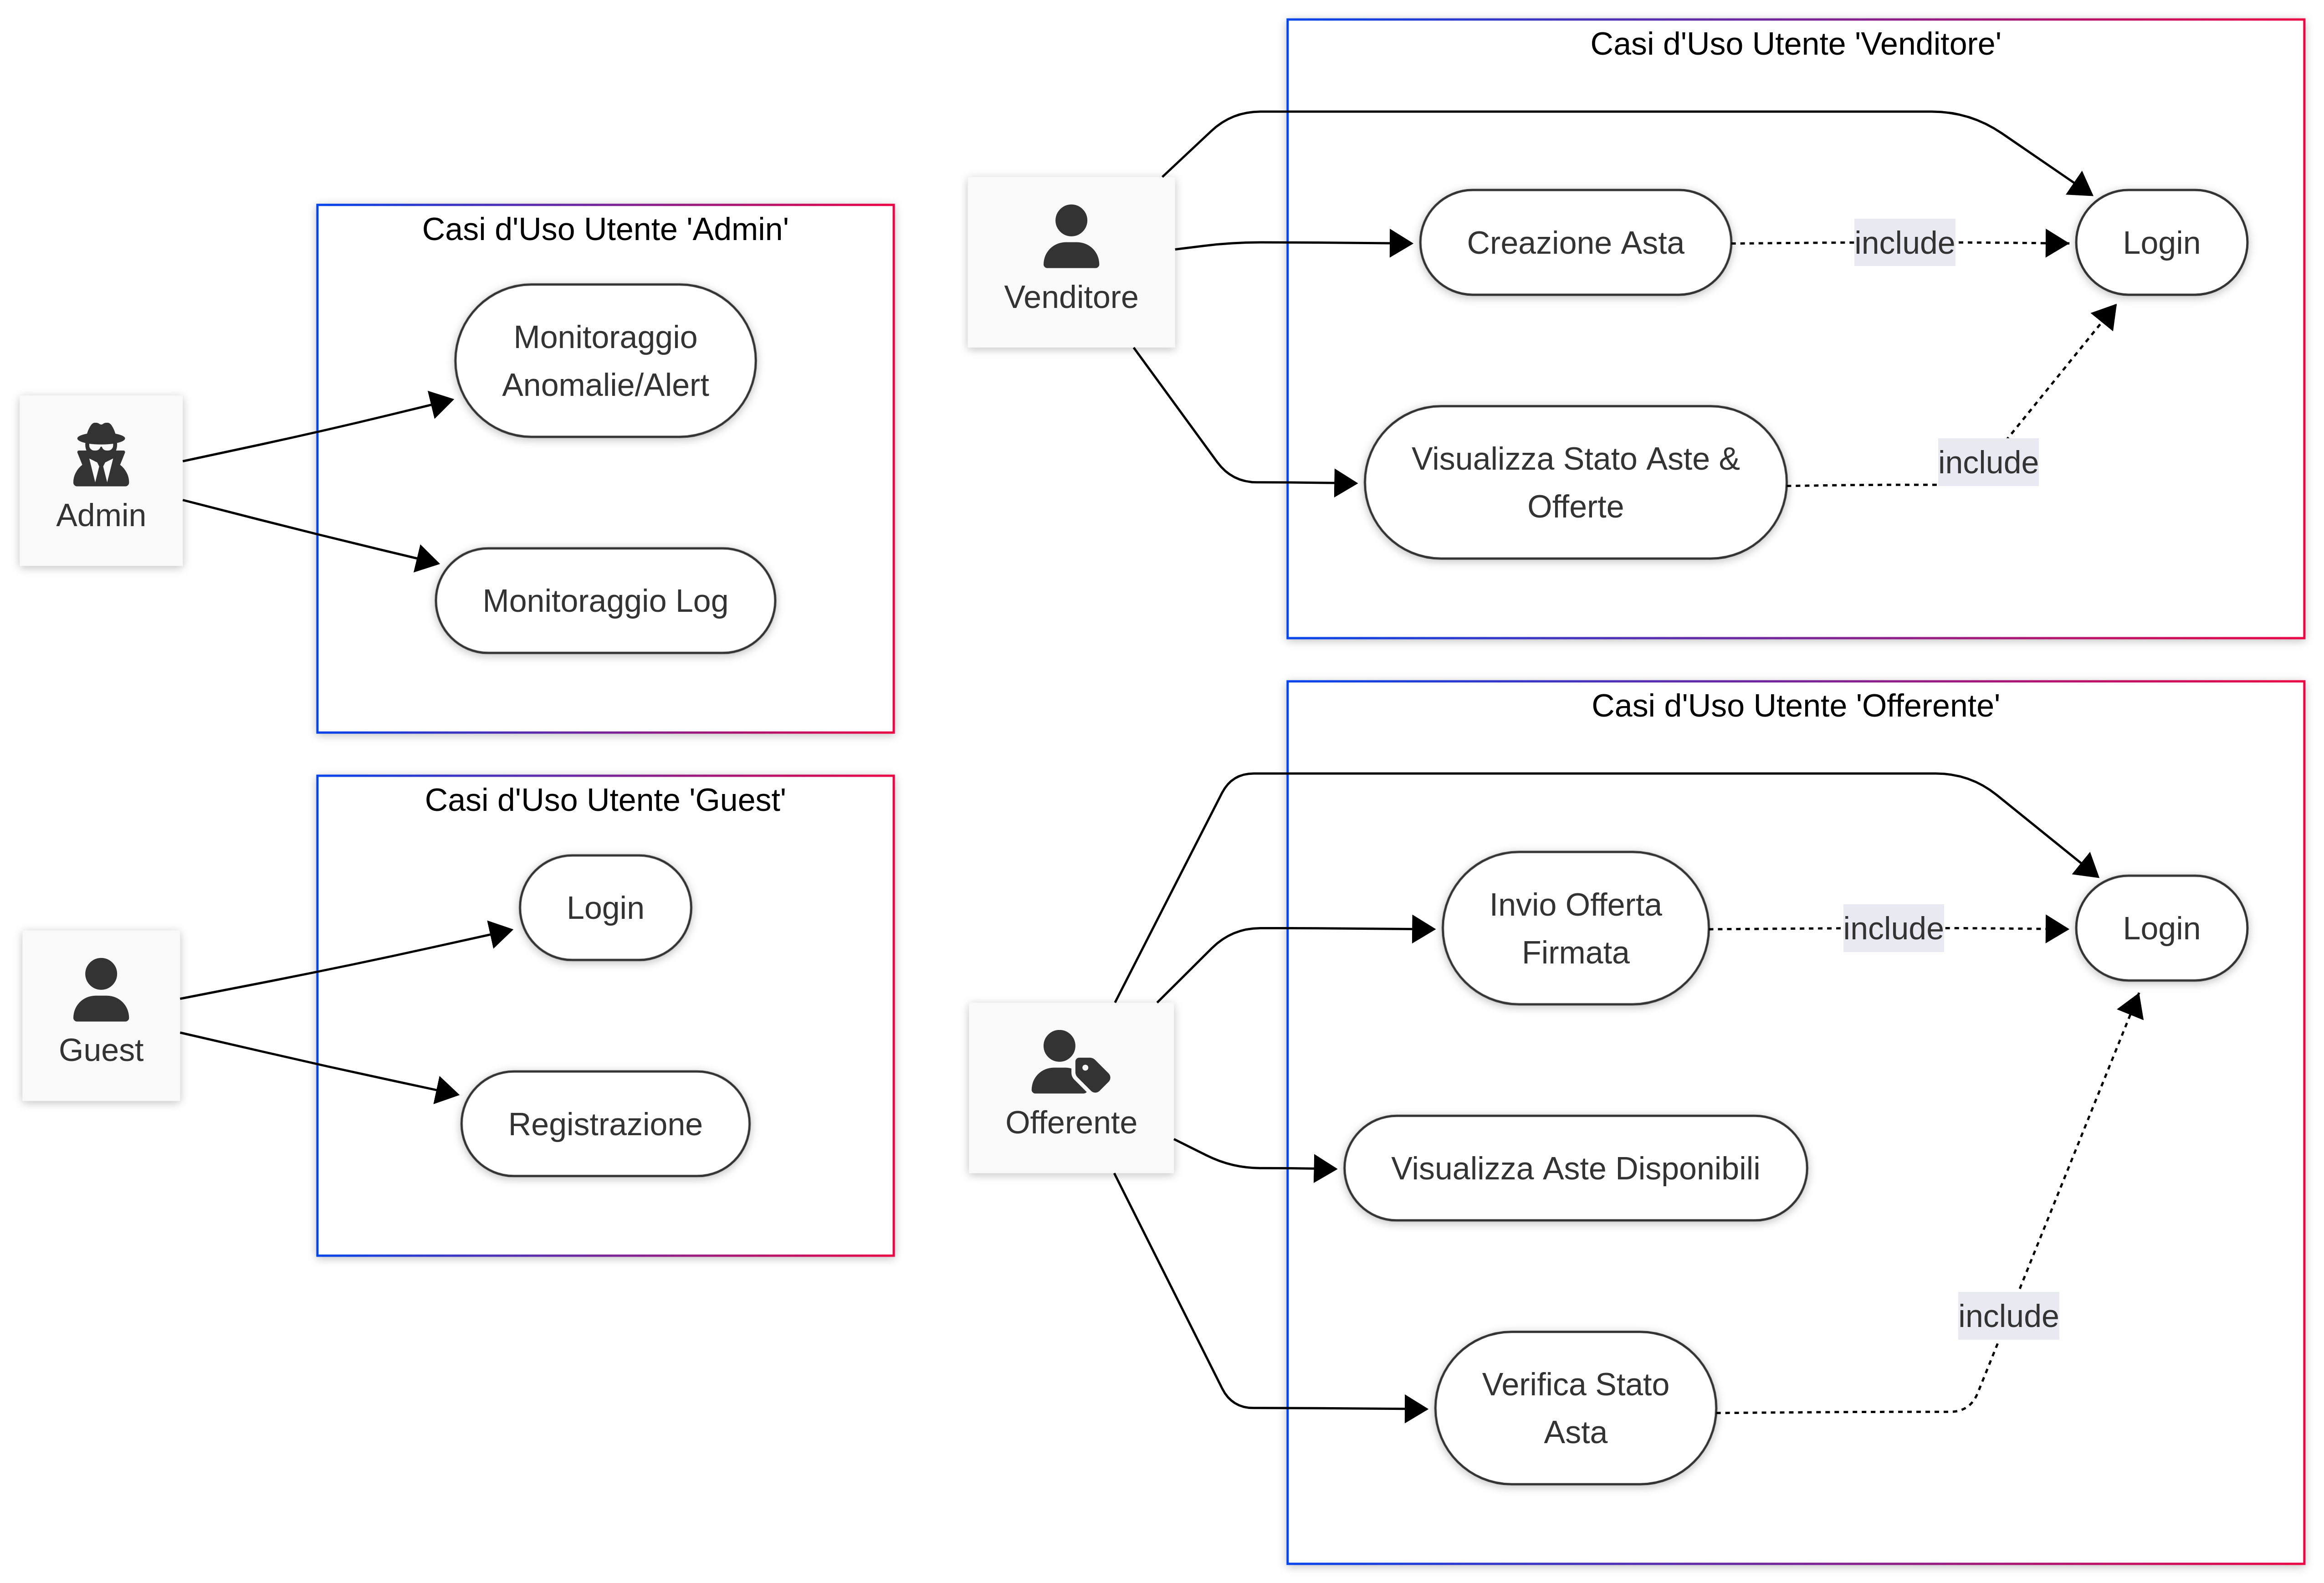
\includegraphics[width=0.75\textwidth]{images/use_cases_users.png}
    \caption{Azioni degli utenti all'interno della piattaforma}
    \label{fig:use_cases}
\end{figure}

\newpage

\section{Frontend}
Per la realizzazione del frontend è stato adottato il motore di templating \textbf{Jinja2} \cite{jinja2}, integrato nativamente in Flask, per la generazione dinamica delle pagine HTML lato server. Jinja2 consente di creare template modulari e riutilizzabili, separando la logica di presentazione dai dati applicativi e facilitando la manutenzione del codice.

Per l'interattività lato client, è stato scelto il framework leggero \textbf{Alpine.js} \cite{alpinejs}, che fornisce reattività senza richiedere una build pipeline complessa. Alpine.js permette di dichiarare il comportamento dinamico direttamente nel markup HTML mediante direttive semplificate, risultando ideale per applicazioni web moderne ma senza la complessità di framework come React o Vue.

Questa combinazione garantisce un frontend performante, mantenibile e facilmente integrabile con il backend Flask, preservando la semplicità dell'architettura complessiva.

Il frontend consiste delle seguenti route:

\begin{description}
    \item[\texttt{/login}] Pagina di autenticazione per l'accesso degli utenti registrati.
    
    \item[\texttt{/signin}] Pagina di registrazione per i nuovi utenti.
    
    \item[\texttt{/}] Pagina home nella quale vengono presentate tutte le aste disponibili in formato grid. Ogni card della griglia mostra la foto principale dell'immobile, il titolo dell'asta, il prezzo di partenza e lo stato. Gli utenti non autenticati possono consultare le aste ma non partecipare.
    
    \item[\texttt{/assets/register}] Pagina dedicata alla registrazione di un nuovo immobile. Un venditore deve fornire le informazioni necessarie quali titolo, ubicazione, descrizione, foto principale e ulteriori dettagli catastali prima di poter procedere alla creazione dell'asta.
    
    \item[\texttt{/auctions/create}] Pagina per la creazione di una nuova asta. Accessibile solo dai venditori che abbiano precedentemente registrato almeno un immobile. Consente di impostare i parametri temporali (data inizio e fine), il prezzo di partenza e l'incremento minimo.
    
    \item[\texttt{/auctions/\{id\}}] Route dinamica generata per ciascun'asta. Visualizza i dettagli completi dell'immobile, lo stato dell'asta in tempo reale, la graduatoria delle offerte (ove applicabile) e consente agli utenti autenticati di partecipare inviando un'offerta.
    
    \item[\texttt{/profile}] Pagina del profilo utente nella quale sono disponibili i dati personali, la cronologia delle aste create (per i venditori) e la cronologia delle offerte inviate (per gli offerenti).
\end{description}

\newpage
\section{Backend (Security Gateway)}

In questa sezione verrà analizzato il backend insieme alla logica di business.
Questa sezione descrive nel dettaglio il componente architetturale che funge da ponte sicuro tra l'interfaccia pubblica (Frontend) e la rete privata (Blockchain Layer). Il Security Gateway non si limita a inoltrare le richieste, ma implementa la logica applicativa necessaria per garantire l'integrità del sistema, la gestione delle identità e la validazione preliminare delle transazioni, proteggendo il Ledger da accessi non autorizzati o malformati.

La tecnologia scelta per l'implementazione del backend è \textbf{Python} \cite{python_software_foundation}, utilizzando il microframework \textbf{Flask} \cite{pallets_flask,flask_jwt_extended}. Questa scelta è motivata dalla necessità di avere un ambiente di sviluppo rapido, flessibile e con un ecosistema ricco di librerie per la crittografia e la gestione delle reti. Il server Flask espone una serie di API RESTful che vengono consumate dal client Frontend.

\subsection{Authentication \& Authorization}

La sicurezza di \textbf{BuySellChain} si articola su due livelli distinti ma interconnessi: l'autenticazione degli utenti e la gestione dei permessi operativi.

\begin{itemize}
    \item \textbf{Autenticazione (Identity Verification):} Il Security Gateway agisce come punto d'ingresso unico. Verifica le credenziali dell'utente (username e password) consultando il database off-chain. Una volta validata l'identità, il sistema mappa l'utente Web 2.0 a un'identità digitale riconosciuta dalla rete Fabric, garantendo che ogni operazione sul ledger sia tracciabile e attribuibile a un attore specifico.
    \item \textbf{Autorizzazione (Access Control):} Dopo l'autenticazione, il sistema applica politiche di controllo degli accessi basate sui ruoli (RBAC). Il backend verifica se l'utente possiede i privilegi necessari per invocare specifiche transazioni (es. solo un utente con ruolo "Venditore" può inizializzare un'asta).
\end{itemize}
    
Il Security Gateway funge da \textit{Policy Enforcement Point}, intercettando le richieste e verificando che il richiedente possieda i privilegi necessari (es. solo il proprietario di un asset può metterlo all'asta) prima di inoltrare qualsiasi comando alla Blockchain.

Una volta completata con successo la fase di login, il server genera e firma un \textit{JSON Web Token} (JWT) \cite{JWTrfc7519}. Questo token funge da passaporto digitale per l'utente e contiene, nel suo \textit{payload}, informazioni essenziali quali l'identificativo utente, i ruoli assegnati e la data di scadenza della sessione.

Il client (Frontend) riceve il token e lo memorizza in modo sicuro. Per ogni successiva interazione con le API del sistema, il client deve includere il JWT nell'header della richiesta HTTP (solitamente nell'header \texttt{Authorization: Bearer <token>}). Questo meccanismo \textit{stateless} permette al backend di validare l'identità del richiedente e verificare le autorizzazioni per ogni singola operazione senza dover interrogare continuamente il database delle credenziali.

\begin{figure}[h!]
    \centering
    \includegraphics[width=1\textwidth]{images/login_seq.png}
    \caption{Flusso di autenticazione/autorizzazione}
    \label{fig:login}
\end{figure}

\newpage

\subsection{Modello Dati \& Interfaccia RESTful API}

Poiché Hyperledger Fabric mantiene il world state come mappa di coppie \texttt{(key, value)}, a livello applicativo è necessario definire: convenzioni di naming per le chiavi (namespace e identificatori), classi/entità applicative e un formato di serializzazione deterministico (es. JSON).

Le API di base fornite dal prof. Arcieri sono pubblicate come endpoint REST. Il Security Gateway riceve le richieste HTTP della piattaforma web e le traduce in comandi per il client Lisp verso la rete Fabric. Ad esempio, una chiamata \texttt{HTTP POST /api/v1/make\_bid} viene mappata al comando \texttt{AddKV}. Il client invoca quindi le funzioni di \emph{chaincode} per creare, leggere, aggiornare o eliminare coppie \texttt{(key, value)} sul ledger.

Le primitive disponibili sono:

\begin{description}
    \item[\texttt{AddKV}:] Inserisce una nuova coppia \texttt{(key, value)} in una classe applicativa.
    \item[\texttt{GetKV}:] Restituisce il \texttt{value} associato a una \texttt{key} di una classe.
    \item[\texttt{GetKeyHistory}:] Restituisce la cronologia immutabile delle operazioni su una \texttt{key}.
    \item[\texttt{DelKV}:] Elimina la coppia \texttt{(key, value)} associata a una \texttt{key}.
    \item[\texttt{GetClasses}:] Restituisce l'elenco delle classi disponibili.
    \item[\texttt{GetNumKeys}:] Restituisce il numero di coppie presenti in una classe.
    \item[\texttt{GetKeys}:] Restituisce l'elenco delle chiavi presenti in una classe.
\end{description}

\begin{lstlisting}[language=json, caption={Envelope di richiesta alle API base}]
{
    ||"cmd"||: "AddKV | GetKV | GetKeyHistory | DelKV | GetClasses | GetNumKeys | GetKeys",
    ||"class"||: "NomeClasse",
    ||"key"||: ["NAMESPACE", "ID"],
    ||"value"||: { ... }
}
\end{lstlisting}

\subsubsection{Definizione Modello Dati}

Di seguito vengono presentate le definizioni strutturali delle classi dati che costituiscono il modello di persistenza distribuito. Ogni tabella rappresenta un'entità logica memorizzata in modo immutabile sulla Blockchain, specificando i campi, i tipi di dato e le relazioni chiare necessarie per garantire l'integrità referenziale e la tracciabilità delle operazioni di compravendita immobiliare all'interno del Ledger di Hyperledger Fabric.

\renewcommand{\arraystretch}{1.2} % Aumenta lo spazio tra le righe
\begin{table}[h!]
    \centering
    \begin{tabular}{@{}llp{6cm}@{}}
        \toprule
        \textbf{Campo} & \textbf{Tipo} & \textbf{Note} \\
        \midrule
        \texttt{id} & string & Identificativo univoco \\
        \texttt{ownerId} & string & Riferimento all'utente proprietario \\
        \texttt{title} & string & Titolo descrittivo immobile \\
        \texttt{location} & string & Indirizzo fisico \\
        \texttt{description} & string & Descrizione immobile \\
        \texttt{currentAuctionId} & string | null & ID dell'asta attiva (se presente) \\
        \texttt{createdAt} & int (epoch) & Data creazione \\
        \texttt{status} & enum & \texttt{ACTIVE}, \texttt{LOCKED}, \texttt{TRANSFERRED} \\
        \bottomrule
    \end{tabular}
    \caption{Definizione della Classe Asset}
\end{table}

\begin{table}[h!]
    \centering
    \begin{tabular}{@{}llp{6cm}@{}}
        \toprule
        \textbf{Campo} & \textbf{Tipo} & \textbf{Note} \\
        \midrule
        \texttt{id} & string & Identificativo univoco offerta \\
        \texttt{auctionId} & string & Riferimento all'asta \\
        \texttt{bidderId} & string & Riferimento all'offerente \\
        \texttt{amount} & number & Importo offerto \\
        \texttt{timestamp} & int (epoch) & Data e ora offerta \\
        \texttt{status} & enum & \texttt{ACCEPTED}, \texttt{REJECTED} \\
        \texttt{rejectReason} & string | null & Motivo del rifiuto (se applicabile) \\
        \bottomrule
    \end{tabular}
    \caption{Definizione della Classe Bid}
\end{table}

\begin{table}[h!]
    \centering
    \begin{tabular}{@{}llp{6cm}@{}}
        \toprule
        \textbf{Campo} & \textbf{Tipo} & \textbf{Note} \\
        \midrule
        \texttt{id} & string & Identificativo univoco dell'asta \\
        \texttt{assetId} & string & Riferimento all'asset in vendita \\
        \texttt{sellerId} & string & Riferimento al venditore \\
        \texttt{startTime} & int (epoch) & Data inizio asta \\
        \texttt{endTime} & int (epoch) & Data fine asta \\
        \texttt{startPrice} & number & Prezzo di partenza \\
        \texttt{minIncrement} & number & Incremento minimo rilancio \\
        \texttt{highestBidId} & string | null & ID dell'offerta vincente attuale \\
        \texttt{highestBidAmount} & number | null & Importo dell'offerta vincente \\
        \texttt{bidsCount} & int & Contatore totale offerte \\
        \texttt{status} & enum & \texttt{ACTIVE}, \texttt{CLOSED}, \texttt{CANCELLED} \\
        \bottomrule
    \end{tabular}
    \caption{Definizione della Classe Auction}
\end{table}

Pertanto, ipotizzando un'analogia con le \textit{tabelle SQL} per fini rappresentativi, la struttura delle classi può essere visualizzata come nello schema seguente:

\begin{figure}[h!]
    \centering
    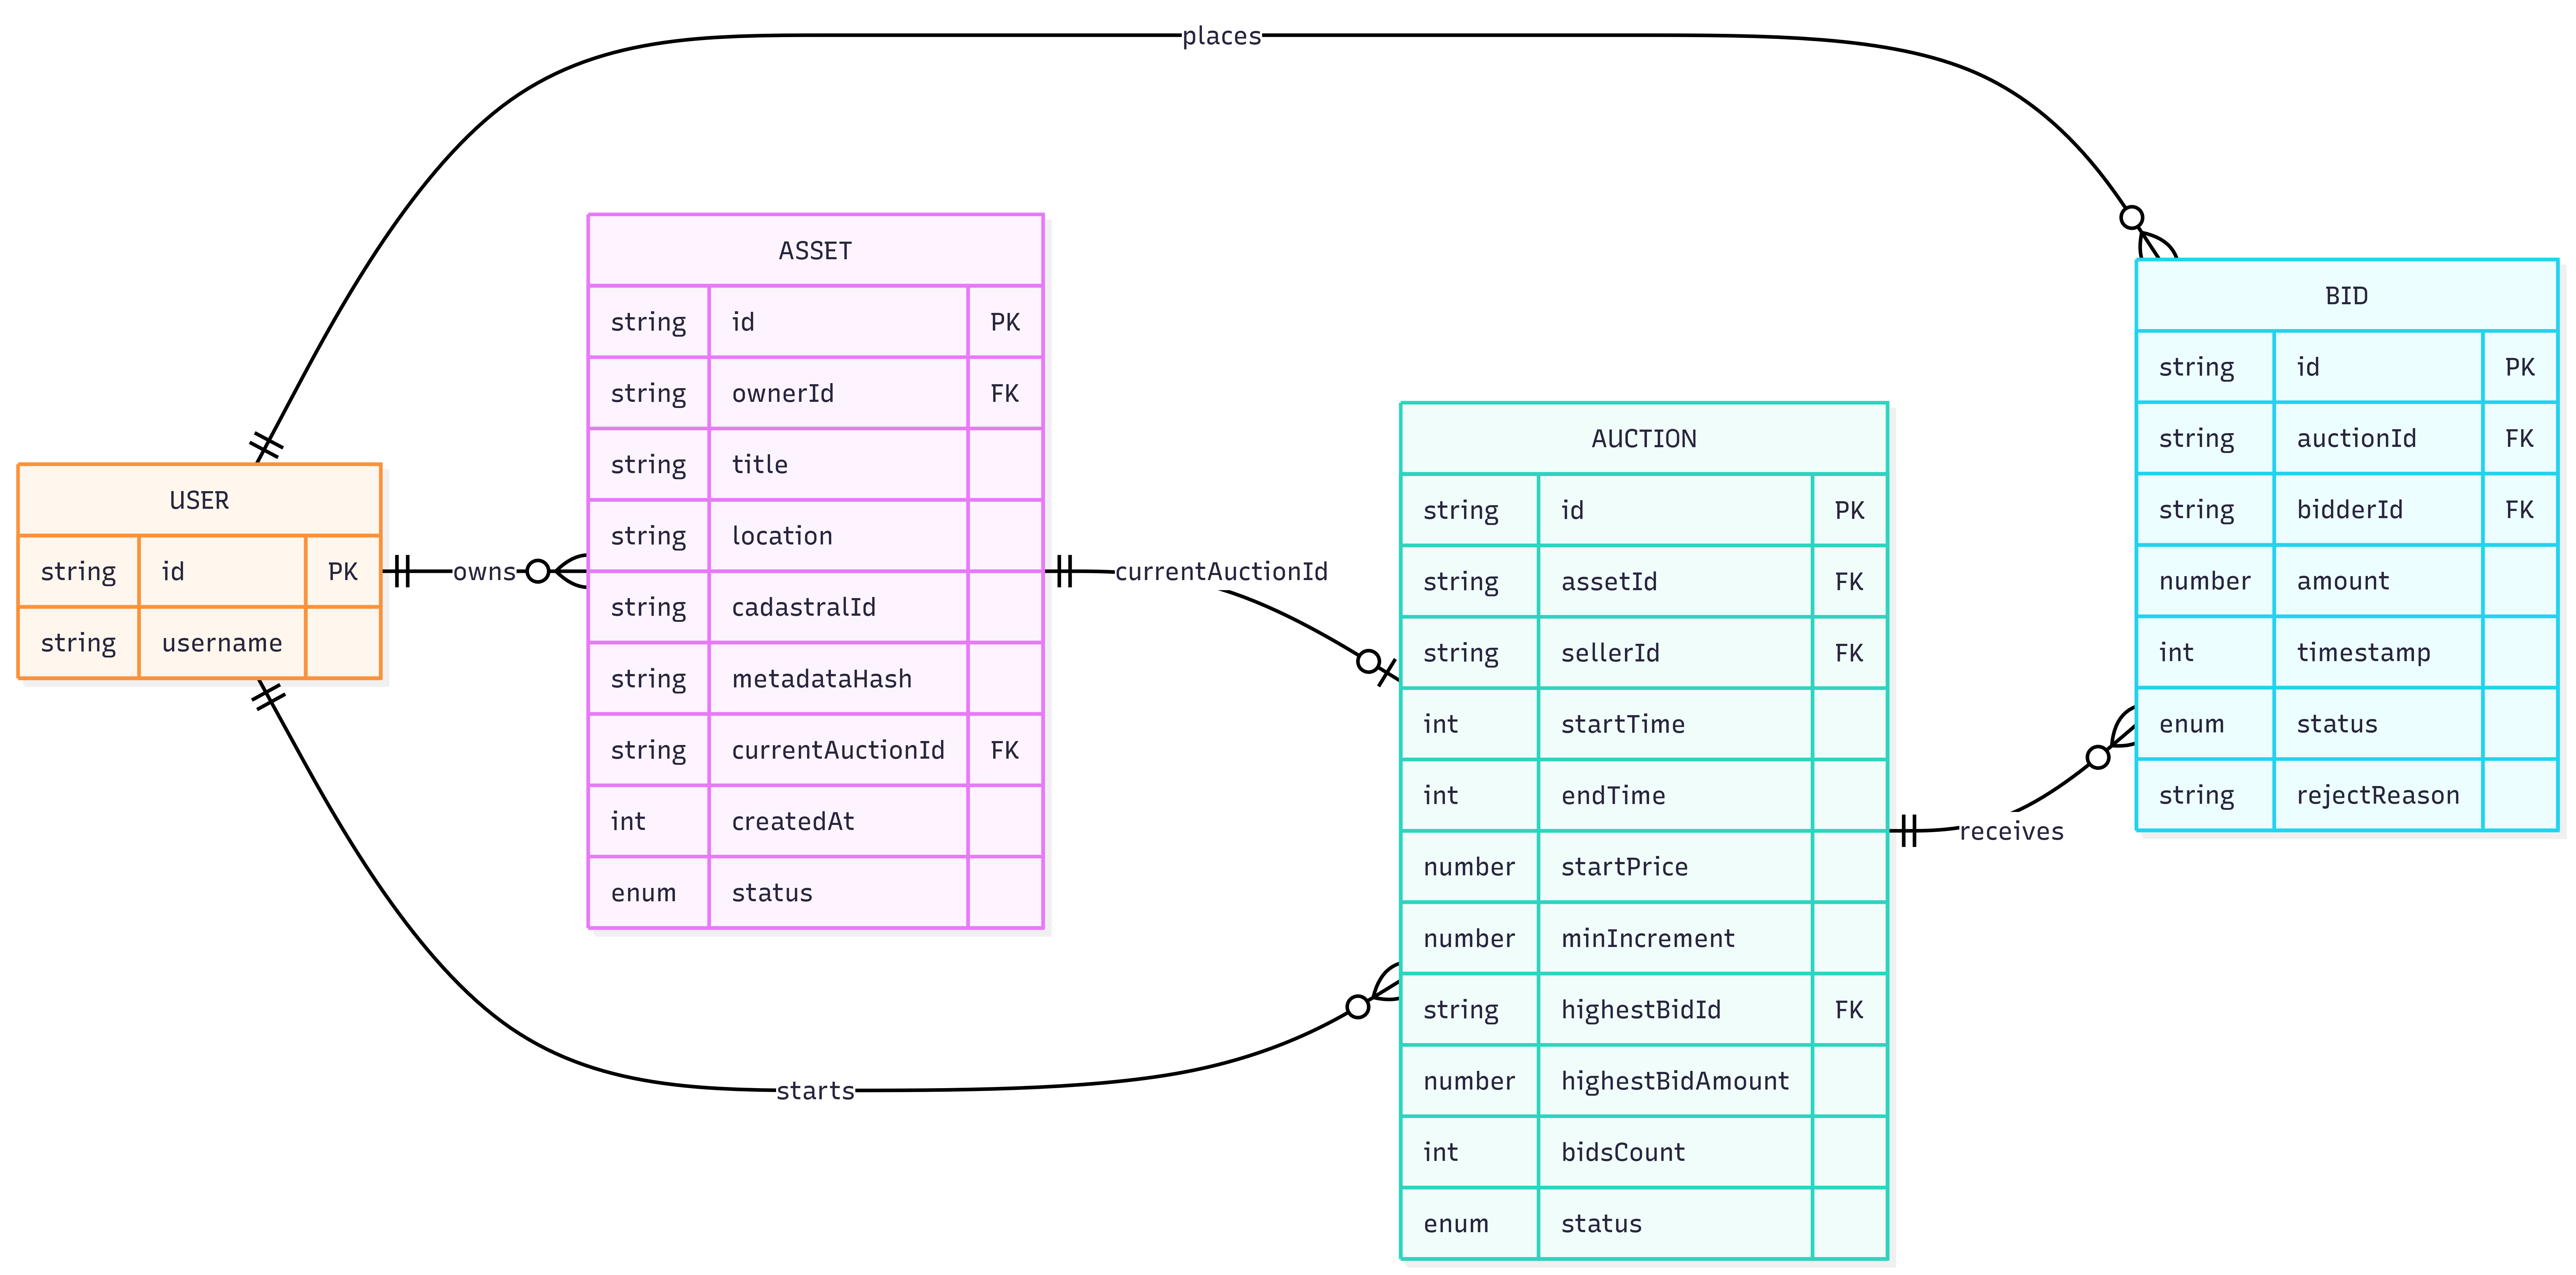
\includegraphics[width=1\textwidth]{images/er_blockchain.png}
    \caption{Schema logico delle tabelle su Fabric}
    \label{fig:er}
\end{figure}

La figura illustra le relazioni logiche tra le entità. L'utente (User) è l'attore principale: può possedere molteplici Asset, avviare diverse Auction e partecipare attivamente inviando Bid. Gli Asset possono essere associati a una Auction attiva (relazione 1:1 opzionale), mentre ogni Auction è legata univocamente a un bene specifico e funge da contenitore per tutte le offerte ricevute.

Questo modello relazionale, pur essendo implementato su un archivio chiave-valore non relazionale, è progettato per garantire la completa tracciabilità della filiera di vendita (provenance). Mantenendo riferimenti incrociati tra venditori, offerenti, beni e stati delle aste, il sistema permette di ricostruire in modo deterministico e immutabile l'intera cronologia di una transazione immobiliare, dall'inserimento dell'asset fino all'aggiudicazione finale, assicurando così la massima trasparenza e integrità dei dati.

\subsubsection{Definizione Interfaccia RESTful API}

Definita la struttura logica dei dati, il passo successivo consiste nell'esposizione dell'interfaccia RESTful API. Nella fase attuale di sviluppo (sperimentale), il server Web è configurato per l'ascolto sulla porta locale standard 5000. L'endpoint base per tutte le richieste API è:
\[
    \texttt{http://localhost:5000/api/v1/}
\]
Per ridurre la complessità infrastrutturale in ambiente di test, la comunicazione avviene attualmente su protocollo HTTP non cifrato.

I principali endpoint sono:

\begin{description}
    \item[\texttt{POST /auth/signin}] 
    Registrazione di un nuovo utente. La richiesta crea un'identità sul database off-chain.
    
    \item[\texttt{POST /auth/login}] 
    Autenticazione utente. Verifica le credenziali e restituisce il token JWT necessario per autorizzare le chiamate successive.
    
    \item[\texttt{POST /assets}] 
    Registrazione di un nuovo immobile sul ledger. Richiede che l'utente sia autenticato e abbia il ruolo di "Venditore". Internamente invoca \texttt{AddKV} per la classe \texttt{Asset}.
    
    \item[\texttt{GET /assets/}] 
    Recupero dettagli di tutti gli assets. Internamente invoca GetKeys e KetKV per la classe omonima.

    \item[\texttt{GET /assets/\{id\}}] 
    Recupero dettagli di uno specifico asset. Internamente invoca \texttt{GetKV} per la classe omonima.
    
    \item[\texttt{POST /auctions}] 
    Creazione di una nuova asta per un asset posseduto dall'utente. Il sistema verifica la proprietà dell'asset e imposta lo stato iniziale dell'asta. Invoca \texttt{AddKV} per la classe \texttt{Auction}.
    
    \item[\texttt{GET /auctions}] 
    Elenco delle aste attive. Supporta filtri opzionali per stato o range di prezzo. Internamente utilizza \texttt{GetKeys} o query specifiche se supportate.
    
    \item[\texttt{POST /bids}] 
    Invio di un'offerta per un'asta attiva. La logica di backend verifica che l'asta sia aperta, che l'offerta superi l'importo corrente più l'incremento minimo, e che l'offerente non sia il venditore stesso. Se valida, registra l'offerta tramite \texttt{AddKV} sulla classe \texttt{Bid} e aggiorna lo stato dell'asta.
    
    \item[\texttt{GET /admin/users}] 
    Restituisce l'elenco completo degli utenti registrati nel database off-chain e il loro stato (attivo/sospeso), per permettere all'amministratore di gestire le utenze.

    \item[\texttt{GET /admin/stats}] 
    Fornisce metriche aggregate del sistema, come il numero totale di aste concluse, il volume delle transazioni e il numero di asset registrati, invocando \texttt{GetNumKeys} sulle diverse classi.

    \item[\texttt{GET /admin/history/\{key\}}] 
    Endpoint di auditing che espone la cronologia immutabile di una specifica chiave (asset o asta), invocando la primitiva \texttt{GetKeyHistory} del chaincode.
\end{description}

\newpage

\begin{lstlisting}[language=json, caption={Esempio di richiesta AddKV per aggiungere un Asset}]
{
    ||"cmd"||: "AddKV",
    ||"class"||: "Asset",
    ||"key"||: ["ASSET", "ASSET_1"],
    ||"value"||: {
        ||"id"||: "ASSET_1",
        ||"ownerId"||: "USER_123",
        ||"title"||: "Villa sul mare",
        ||"location"||: "Via del lungomare 12",
        ||"cadastralId"||: "a7bbcecb",
        ||"metadataHash"||: "e5990593c22e6647a7bbde8e85f395e56727a7bbd8ccecb6",
        ||"currentAuctionId"||: "AUCTION_2",
        ||"createdAt"||: 1769509800,
        ||"status"||: "LOCKED"
    }
}
\end{lstlisting}

\begin{lstlisting}[language=json, caption={Esempio di richiesta AddKV per creare un'asta}]
{
    ||"cmd"||: "AddKV",
    ||"class"||: "Auction",
    ||"key"||: "auction:AUCTION_2",
    ||"value"||: {
        ||"id"||: ["AUCTION", "AUCTION_2"],
        ||"assetId"||: "ASSET_1",
        ||"sellerId"||: "USER_123",
        ||"startTime"||: 1769509200,
        ||"endTime"||: 1769516400,
        ||"startPrice"||: 350000,
        ||"minIncrement"||: 5000,
        ||"highestBidId"||: null,
        ||"highestBidAmount"||: null,
        ||"bidsCount"||: 0,
        ||"status"||: "ACTIVE"
    }
}
\end{lstlisting}


\begin{lstlisting}[language=json, caption={Esempio di richiesta AddKV per aggiungere un'offerta (Bid)}]
{
    ||"cmd"||: "AddKV",
    ||"class"||: "Bid",
    ||"key"||: ["bid", "BID_1"],
    ||"value"||: {
        ||"id"||: "BID_1",
        ||"auctionId"||: "AUCTION_2",
        ||"bidderId"||: "USER_456",
        ||"amount"||: 355000,
        ||"timestamp"||: 1769509500,
        ||"status"||: "ACCEPTED",
        ||"rejectReason"||: null
    }
}
\end{lstlisting}

\subsection{Logica di Bussiness}

La piattaforma implementa un modello di gestione degli attori e delle aste articolato in fasi distinte:

\paragraph{Registrazione e Verifica dei Venditori}
Un utente che desideri partecipare alle aste come venditore deve completare una procedura di registrazione qualificata. Oltre alle informazioni anagrafiche standard (nome, cognome, email, numero di telefono), il sistema richiede l'inserimento del codice fiscale, necessario per garantire l'identificazione univoca e conforme alle normative sulla tracciabilità delle operazioni immobiliari. Una volta sottomessa la richiesta, un messaggio di notifica viene inviato agli amministratori del sistema, i quali hanno la responsabilità di validare l'identità del richiedente e approvare o rifiutare l'iscrizione al ruolo di venditore.

\paragraph{Struttura Temporale delle Aste}
Ogni asta è caratterizzata da un intervallo temporale definito dal venditore, durante il quale gli offerenti possono partecipare. Tale intervallo è suddiviso logicamente in finestre temporali di durata predeterminata, al fine di implementare meccanismi anti-frontrunning e garantire equità nella partecipazione.

\paragraph{Vincoli sulle Offerte}
Per ogni finestra temporale, ciascun offerente può inviare al massimo una sola offerta. Questa limitazione impedisce comportamenti speculativi e riduce la complessità computazionale del sistema. Le offerte rimangono nascoste agli altri partecipanti fino al termine della relativa finestra temporale, garantendo così l'anonimato del processo di bidding.

\paragraph{Aggiornamento dello Stato dell'Asta}
Al termine di ogni finestra temporale, il sistema esegue automaticamente un'operazione di consolidamento dello stato dell'asta:
\begin{itemize}
    \item Vengono valutate tutte le offerte ricevute durante la finestra.
    \item I campi \texttt{highestBidAmount} e \texttt{bidsCount} vengono aggiornati per riflettere l'offerta vincente e il conteggio totale.
    \item Lo stato dell'asta transisce in \texttt{LOCKED}, impedendo temporaneamente l'invio di nuove offerte.
    \item Il venditore acquisisce la possibilità di modificare il parametro \texttt{minIncrement}, adattando dinamicamente il valore richiesto per i successivi rilanci.
\end{itemize}
Una volta completato l'aggiornamento, l'asta ritorna allo stato \texttt{ACTIVE}, rendendo di nuovo disponibile la partecipazione per la finestra temporale successiva.

L'intervallo temporale compreso tra \texttt{startTime} e \texttt{endTime} viene suddiviso in finestre temporali discrete secondo il seguente schema:

\[
    \mathrm{window\_duration} = \frac{\mathrm{endTime} - \mathrm{startTime}}{n}
\]

dove $n$ rappresenta il numero totale di finestre temporali configurabili dal venditore al momento dell'inizializzazione dell'asta. Questo meccanismo garantisce una distribuzione equa degli intervalli di partecipazione e facilita l'implementazione di politiche anti-frontrunning, in quanto ogni finestra temporale costituisce un perimetro di validazione indipendente per le offerte ricevute.

\newpage
\section{Blockchain Layer}
L'ultimo layer dell'architettura è rappresentato dalla blockchain Hyperledger Fabric, che svolge due ruoli fondamentali nel sistema: fungere da database distribuito e immutabile, e validare le transazioni effettuate dagli utenti secondo le regole definite negli Smart Contract.

In questo contesto, Fabric agisce come sistema di registrazione ufficiale (ledger) per tutte le operazioni critiche di compravendita: dalla registrazione degli asset immobiliari, alla creazione delle aste, fino alla registrazione delle offerte. La natura distribuita e permissioned della rete garantisce che ogni transazione sia validata da più peer secondo il meccanismo di consenso configurato, assicurando così l'integrità e la non-ripudiabilità delle operazioni.

Il Security Gateway comunica con la rete Fabric esclusivamente tramite il client Lisp fornito dal docente, che incapsula la logica di interazione con il chaincode e la gestione delle identità crittografiche (MSP). Questo isolamento protegge il ledger da accessi diretti e non autorizzati.

\begin{figure}[h!]
    \centering
    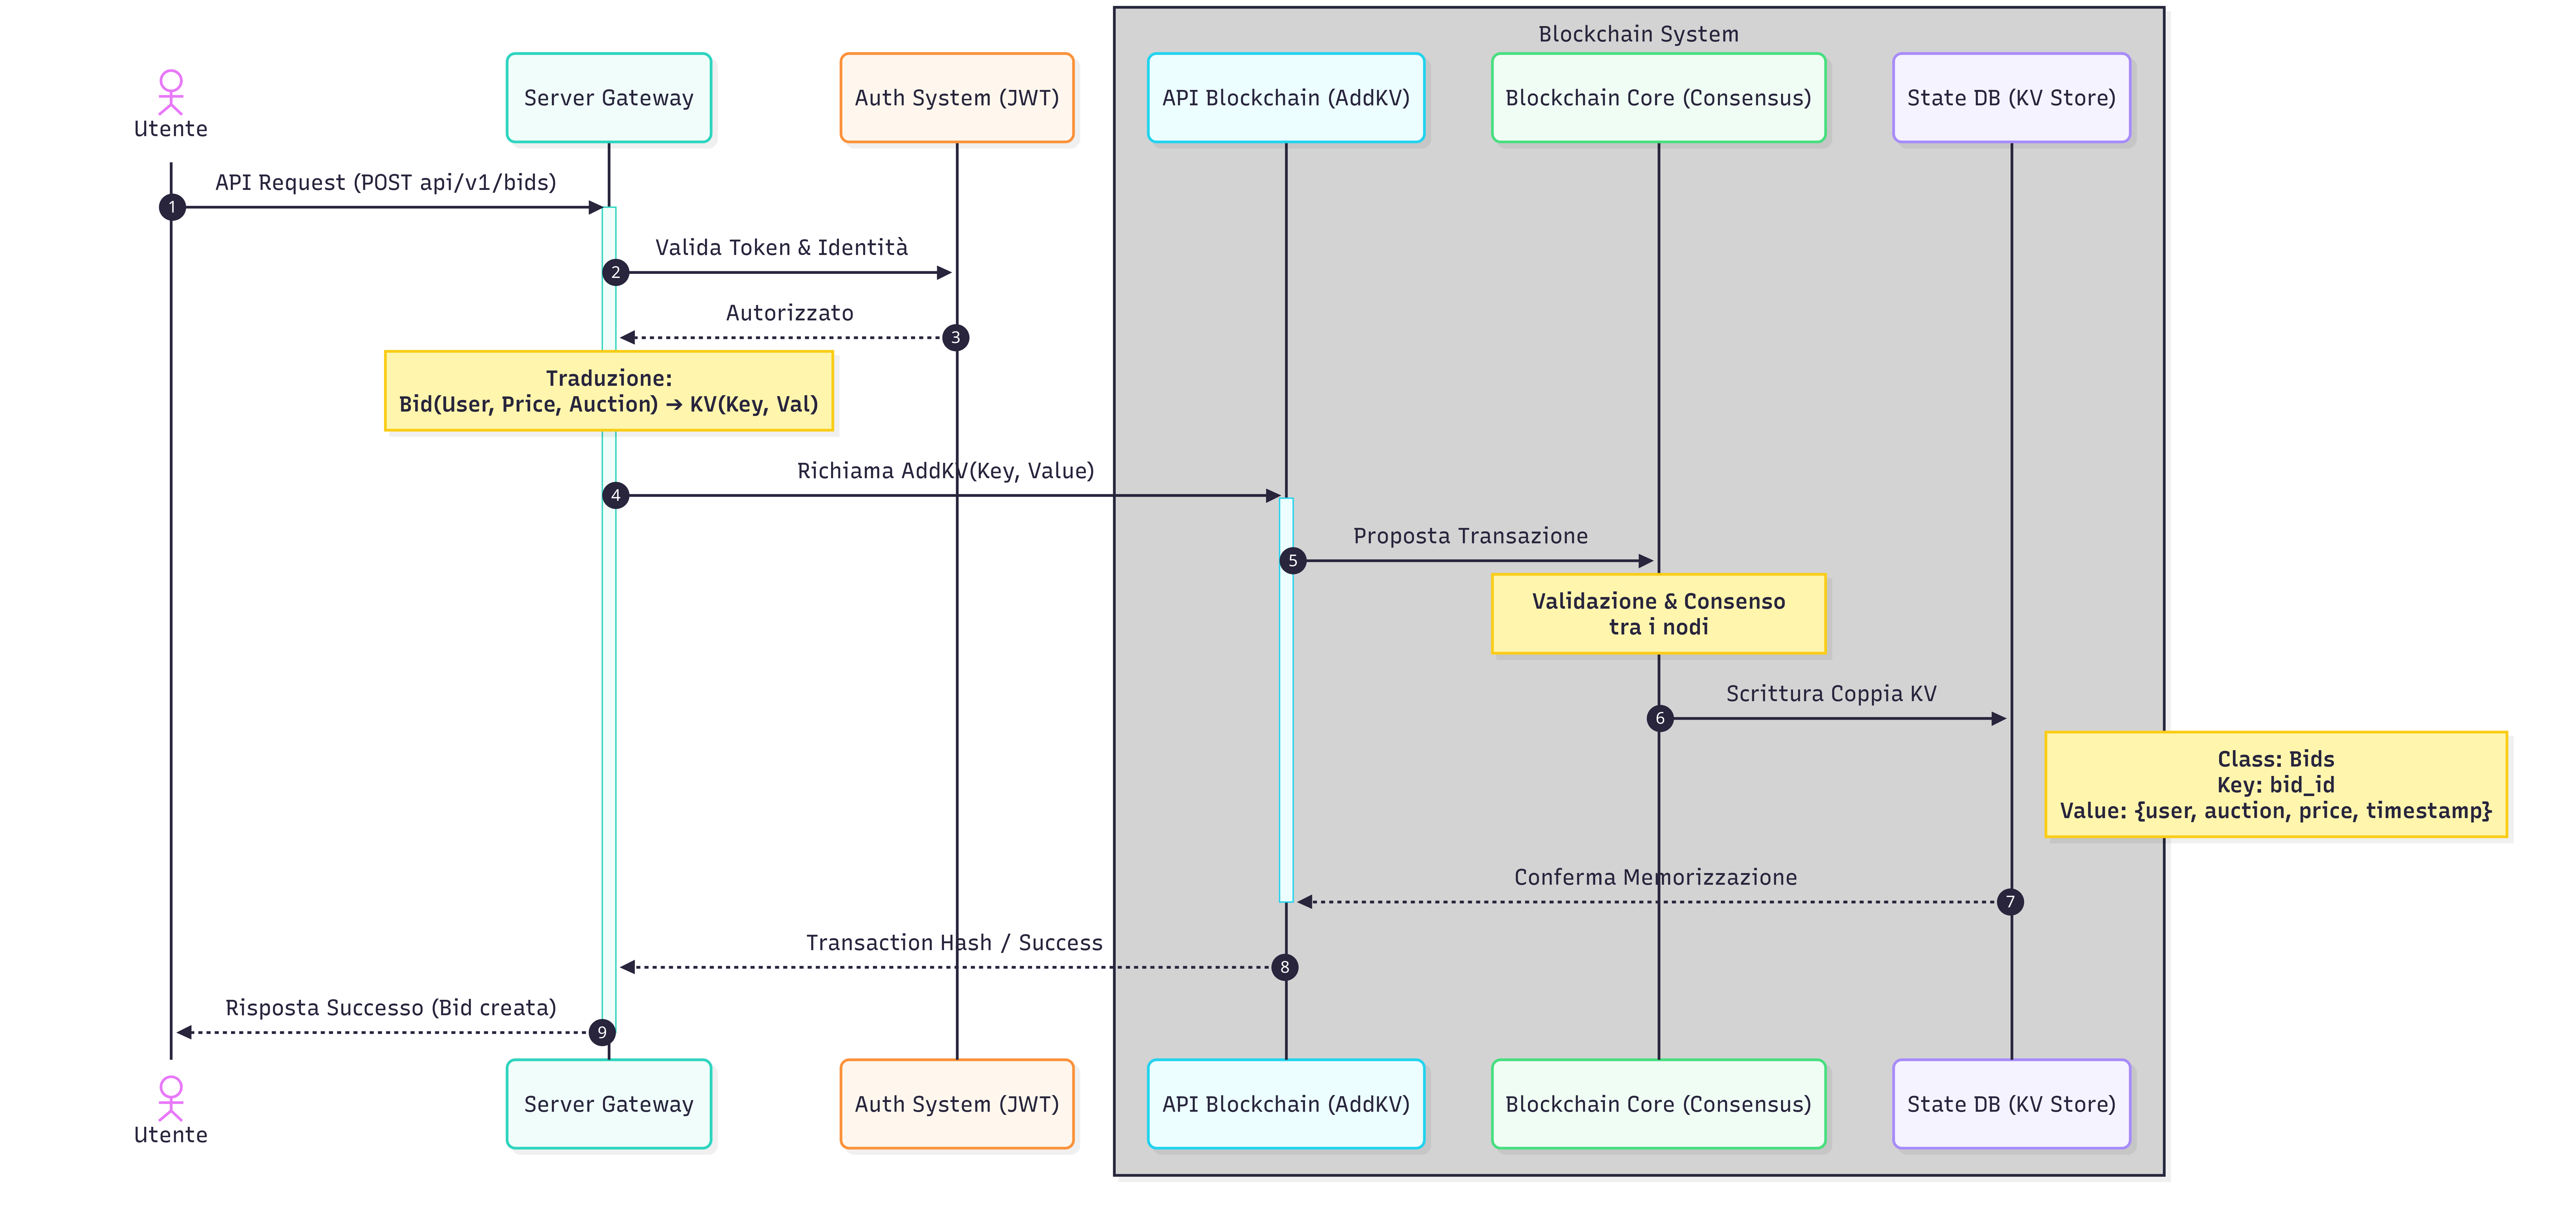
\includegraphics[width=1\textwidth]{images/make_bid_seq.png}
    \caption{Flusso di azioni per la creazione di un'offerta}
    \label{fig:make_bid_seq}
\end{figure}

\newpage
\section{Database Off-Chain}

Il database off-chain è responsabile della persistenza dei dati sensibili e delle informazioni anagrafiche degli utenti, garantendo che tali dettagli non vengano esposti direttamente sul Ledger immutabile. Il Security Gateway interagisce con questo componente per validare le credenziali di accesso e gestire i permessi, fungendo da ponte tra l'identità dell'utente sulla piattaforma web e il suo corrispettivo crittografico sulla rete Blockchain. La tecnologia adottata per l'implementazione è PostgreSQL \cite{postgresql}.

\begin{table}[h!]
    \centering
    \begin{tabular}{lll}
        \hline
        Campo & Tipo & Note \\
        \hline
        \texttt{id} & string & allineato a \texttt{user:<uuid>} on-chain \\
        \texttt{role} & array di enum & \texttt{ADMIN}, \texttt{SELLER}, \texttt{BIDDER} \\
        \texttt{name} & string & \\
        \texttt{surname} & string & \\
        \texttt{email} & string & \\
        \texttt{birthday} & date & \\
        \texttt{cellularNumber} & number & \\
        \texttt{passwordHash} & string & \\
        \texttt{lastLoginAt} & int (epoch) & \\
        \texttt{createdAt} & int (epoch) & \\
        \hline
    \end{tabular}
    \caption{Tabella Users}
\end{table}

Per l'interazione con PostgreSQL nel contesto del framework Flask, è stata adottata la libreria \textbf{SQLAlchemy} \cite{sqlalchemy}, un'astrazione Object-Relational Mapping (ORM) che consente di operare su query strutturate anziché ricorrere a SQL puro. Questo approccio garantisce una maggiore sicurezza nei confronti di attacchi SQL injection e una migliore manutenibilità del codice.

Al fine di semplificare la gestione dell'infrastruttura di sviluppo e garantire la portabilità dell'applicazione, il database PostgreSQL è stato containerizzato mediante \textbf{Docker}. La configurazione del container è definita in un file \texttt{docker-compose.yml}, il quale specifica i parametri di connessione, il volume di persistenza dei dati e le variabili di ambiente necessarie. Questo approccio consente agli sviluppatori di avviare l'intera stack del database con un singolo comando, eliminando le dipendenze dall'ambiente locale e facilitando il deployment su sistemi eterogenei.

Per la messa in sicurezza delle credenziali è stato adottato l'algoritmo di hashing crittografico bcrypt, basato sul cifrario Blowfish. Il processo integra nativamente la generazione di un salt univoco per ogni utente, restituendo una stringa finale che concatena versione, costo, salt e digest secondo la struttura:
\[
    \texttt{pwd\_hash}=\$2b\$[\texttt{cost}]\$[\texttt{salt}]\$[\texttt{hash}]
\]
Questo approccio garantisce protezione contro attacchi di tipo rainbow table e attacchi a forza bruta grazie al fattore di costo adattivo.

\cleardoublepage
\phantomsection
\chapter{Superficie osservabile e Perimetro di Attacco}

L'architettura di \texttt{BuySellChain} adotta un approccio ibrido che integra la flessibilità del Web 2.0 con la sicurezza decentralizzata del Web 3.0. Questa disaccoppiatura tra il Security Gateway, il database off-chain e il ledger distribuito su Hyperledger Fabric offre robuste garanzie architettoniche, ma espande parallelamente la superficie d'attacco. Un potenziale avversario potrebbe sfruttare vulnerabilità in diversi punti di contatto tra questi layer. Di seguito viene delineato in dettaglio il perimetro d'attacco, analizzando i possibili vettori di minaccia per ciascun livello dell'infrastruttura.

\section{Livello Client (Frontend)}
Il frontend, realizzato con i template Jinja2 e il framework Alpine.js, rappresenta il punto di interazione primario per gli utenti autenticati e non autenticati. Sebbene non contenga logica di business critica, è esposto a vulnerabilità tipiche delle applicazioni web lato client:

\begin{itemize}
    \item \textbf{Cross-Site Scripting (XSS):} Poiché il frontend genera pagine HTML dinamiche tramite Jinja2, un'inadeguata sanitizzazione degli input dell'utente (ad esempio nella descrizione di un immobile o nei parametri di registrazione) potrebbe permettere a un attaccante di iniettare script JavaScript malevoli. Se eseguiti nel browser di un'altra vittima, questi script potrebbero sottrarre informazioni sensibili.
    \item \textbf{Furto del Token JWT e Session Hijacking:} A seguito dell'autenticazione, il token JWT viene salvato localmente nel client (LocalStorage o Cookie). Se un attacco XSS dovesse avere successo e il token fosse conservato nel LocalStorage (che non è protetto dal flag \texttt{HttpOnly}), l'attaccante potrebbe rubare il token ed effettuare un \textit{session hijacking}, impersonando l'utente per compiere azioni non autorizzate (es. piazzare offerte fraudolente).
    \item \textbf{Manipolazione dell'Interfaccia e CSRF:} Un utente malintenzionato potrebbe alterare il DOM locale (ad esempio riattivando pulsanti disabilitati per aste chiuse) nel tentativo di inviare payload imprevisti al server. Inoltre, in assenza di header \texttt{Anti-CSRF}, richieste forgiate da domini terzi potrebbero ingannare il browser dell'utente portandolo a eseguire azioni non volute.
\end{itemize}

\section{Livello Application / Security Gateway (Backend)}
Il server applicativo basato su Flask svolge il ruolo di middleware e Policy Enforcement Point. Essendo l'unico componente direttamente esposto alla rete pubblica per filtrare le richieste dirette al ledger, rappresenta il bersaglio primario:

\begin{itemize}
    \item \textbf{Intercettazione Man-in-the-Middle (MiTM):} Nell'attuale configurazione di sviluppo, il server ascolta sulla porta locale 5000 utilizzando il protocollo HTTP non cifrato. Questo espone integralmente il traffico di rete: credenziali in chiaro durante la \texttt{POST /auth/login} e token JWT trasmessi nell'header \texttt{Authorization} sono facilmente intercettabili tramite \textit{packet sniffing}.
    \item \textbf{Bypass dei Controlli di Autorizzazione (RBAC) e Vulnerabilità JWT:} Il sistema fa forte affidamento sui JWT per l'autorizzazione stateless. Se la chiave segreta (HMAC) utilizzata per firmare i token risultasse debole o venisse compromessa, un attaccante potrebbe forgiare token validi alterando il payload per elevare i propri privilegi (ad esempio, assegnandosi il ruolo \texttt{SELLER} o \texttt{ADMIN}). Inoltre, vulnerabilità nell'implementazione della libreria potrebbero permettere attacchi di tipo \textit{signature stripping} (es. forzare l'algoritmo \texttt{none}).
    \item \textbf{Lisp Command Injection e Parameter Tampering:} Il backend traduce le richieste RESTful in primitive per il client Lisp (\texttt{AddKV}, \texttt{GetKV}, \texttt{DelKV}). Qualora la validazione dei JSON in ingresso da parte dell'API fosse carente, un attaccante potrebbe inviare payload malformati (es. chiavi contenenti caratteri di escape non previsti o strutture annidate anomale) tentando di manipolare la query destinata al chaincode o di causare un Denial of Service (DoS) nel parser Lisp.
    \item \textbf{Abuso delle API e Denial of Service (DoS):} L'assenza esplicita di meccanismi di \textit{Rate Limiting} sugli endpoint pubblici (come \texttt{/api/v1/auth/login} o \texttt{/api/v1/bids}) permette ad attaccanti di sferrare attacchi di tipo Brute Force contro gli account degli utenti, o di inondare il sistema di offerte fasulle saturando le risorse di calcolo del Security Gateway e rallentando il consenso della blockchain.
\end{itemize}

\section{Livello Dati Off-Chain (Database PostgreSQL)}
Il database PostgreSQL containerizzato gestisce dati anagrafici sensibili (GDPR) e credenziali:

\begin{itemize}
    \item \textbf{SQL Injection Avanzato:} L'uso dell'ORM SQLAlchemy mitiga gran parte dei rischi di SQL injection standard. Tuttavia, se in qualche punto del codice sorgente venissero utilizzate query SQL raw senza un'adeguata sanitizzazione, un attaccante potrebbe sfruttare questa vulnerabilità per esfiltrare dati sensibili, modificare record o addirittura eseguire comandi arbitrari sul server database.
    \item \textbf{Cracking Off-Line delle Credenziali:} Le password sono protette da hashing \texttt{bcrypt} con salt unico. Se il parametro di costo adattivo (cost factor) fosse configurato su un valore troppo basso per favorire le performance, un attaccante che riuscisse a ottenere un dump del database potrebbe eseguire efficaci attacchi dizionario offline utilizzando hardware dedicato (GPU/ASIC).
    \item \textbf{Vulnerabilità dell'Ambiente Docker (Container Escape):} Il database è distribuito tramite \texttt{docker-compose.yml}. Misconfigurazioni operative, come l'esecuzione del container in modalità \textit{privileged}, l'eccessiva esposizione delle porte (es. esporre la porta 5432 globalmente su \texttt{0.0.0.0} anziché solo al backend), o vulnerabilità non patchate nell'engine di Docker, potrebbero consentire a un aggressore di sfuggire all'isolamento del container e compromettere l'intero server host.
\end{itemize}

% \section{Livello Blockchain e Smart Contract (Hyperledger Fabric)}

% Il cuore del sistema risiede in Hyperledger Fabric, accessibile solo tramite identità crittografiche verificate:

% \begin{itemize}
%     \item \textbf{Compromissione dell'Infrastruttura PKI (MSP/CA):} Il modello \textit{permissioned} di Fabric basa la fiducia sui certificati X.509 emessi dalle CA e validati dai Membership Service Providers (MSP). Se la chiave privata di una Certificate Authority dovesse essere esfiltrata (ad esempio tramite un attacco al server host), l'avversario potrebbe emettere certificati validi per nodi Peer fittizi o amministratori fittizi, compromettendo irreparabilmente l'integrità del ledger e bypassando completamente le difese del Security Gateway.
%     \item \textbf{Vulnerabilità Logiche e Race Conditions nello Smart Contract:} La compravendita è regolata da complesse transizioni di stato (da \texttt{ACTIVE} a \texttt{LOCKED} e poi di nuovo ad \texttt{ACTIVE} al termine di ogni finestra). Se le funzioni del chaincode non garantiscono l'atomicità assoluta o se l'aggiornamento simultaneo di \texttt{highestBidAmount} e dello stato dell'asta soffre di \textit{race conditions}, due offerte arrivate al medesimo istante potrebbero causare un'inconsistenza del \textit{world state}, sovrascrivendo l'offerta legittimamente vincente.
%     \item \textbf{Attacchi di Frontrunning e Manipolazione Temporale:} Il sistema suddivide le aste in finestre temporali definite dalla formula $$window\_duration = \frac{endTime - startTime}{n}$$ per mitigare i comportamenti speculativi. Ciononostante, un attaccante esperto potrebbe monitorare i tempi di propagazione della rete (latency) e sfruttare le lievi derive degli orologi di sistema (clock drift) dei vari nodi \textit{Orderer}. Sottomettendo un'offerta all'esatto limite temporale di chiusura della finestra, potrebbe tentare di includere la propria transazione nel blocco ignorando il vincolo della singola offerta per finestra o prevedendo lo stato invisibile degli altri partecipanti prima del consolidamento.
% \end{itemize}
\chapter{Possibili Attacchi e Contromisure}

Alla luce della superficie d'attacco analizzata nel capitolo precedente, è fondamentale definire una strategia di difesa in profondità (\textit{Defense-in-Depth}). Il sistema \texttt{BuySellChain} deve garantire la confidenzialità, l'integrità e la disponibilità dei dati in ogni layer della sua architettura ibrida. Di seguito vengono descritti in dettaglio gli scenari di attacco più critici e le contromisure tecniche e architetturali adottate per la loro mitigazione.

\section{Difesa del Frontend e Gestione Sicura delle Sessioni}

Il layer di presentazione, pur essendo privo di logica di business, rappresenta il primo punto di contatto con l'utente ed è esposto ad attacchi client-side.

\begin{itemize}
    \item \textbf{Attacco: Cross-Site Scripting (XSS) e Furto di JWT}\\
    Come evidenziato, l'archiviazione del token JWT nel \texttt{LocalStorage} del browser espone il sistema al furto delle sessioni in caso di vulnerabilità XSS.
    \item \textbf{Contromisura: Cookie HttpOnly e CSP}\\
    Per mitigare questo rischio, il Security Gateway è configurato per rilasciare il token JWT esclusivamente tramite un \textit{Cookie} di sessione protetto dai flag \texttt{HttpOnly}, \texttt{Secure} e \texttt{SameSite=Strict}. Il flag \texttt{HttpOnly} rende il cookie invisibile agli script JavaScript eseguiti nel browser (es. Alpine.js o script malevoli), impedendone il furto diretto. Inoltre, viene implementata una rigorosa \textit{Content Security Policy} (CSP) tramite gli header HTTP per restringere le fonti da cui il browser è autorizzato a caricare script esterni, riducendo drasticamente la probabilità di successo di un attacco XSS.
    
    \item \textbf{Attacco: Cross-Site Request Forgery (CSRF)}\\
    L'utilizzo di cookie di sessione reintroduce il rischio di CSRF, dove un sito malevolo potrebbe forzare il browser dell'utente a inviare richieste autenticate al backend di \texttt{BuySellChain}.
    \item \textbf{Contromisura: Token Anti-CSRF}\\
    Viene introdotto un meccanismo di token sincrono (\textit{Synchronizer Token Pattern}). Il server Flask genera un token CSRF univoco per ogni sessione, integrato nei form HTML generati da Jinja2. Ogni richiesta di modifica dello stato (es. \texttt{POST /bids}) deve includere questo token, validato dal backend prima di processare la transazione.
\end{itemize}

\section{Hardening del Security Gateway (Backend)}

Il backend Flask agisce come \textit{Security Gateway} e richiede protezioni rigorose per impedire compromissioni dirette e abusi.

\begin{itemize}
    \item \textbf{Attacco: Man-in-the-Middle (MitM)}\\
    L'utilizzo del protocollo HTTP in chiaro espone le credenziali e le comunicazioni API.
    \item \textbf{Contromisura: Cifratura TLS/SSL (HTTPS)}\\
    In ambiente di produzione, il server Flask non viene esposto direttamente. Viene introdotto un Reverse Proxy (es. NGINX) incaricato di gestire la terminazione TLS. Tutte le comunicazioni tra il client e il sistema sono cifrate forzatamente in HTTPS (TLS 1.3), garantendo la confidenzialità in transito e neutralizzando il \textit{packet sniffing}.
    
    \item \textbf{Attacco: Lisp Command Injection e Payload Malformati}\\
    L'iniezione di caratteri di escape nel JSON potrebbe manipolare le query verso il client Lisp.
    \item \textbf{Contromisura: Validazione Rigorosa degli Input (JSON Schema)}\\
    Prima di invocare le primitive \texttt{AddKV} o \texttt{GetKV}, il backend applica una validazione strutturale e semantica (\textit{Input Sanitization}) tramite \texttt{JSON Schema}. Ogni campo viene tipizzato, limitato in lunghezza e filtrato per rimuovere caratteri non consentiti. Solo i payload conformi allo schema atteso vengono inoltrati alla rete Fabric.
    
    \item \textbf{Attacco: Denial of Service (DoS) e Brute Force}\\
    Inondare gli endpoint di autenticazione o di offerta di richieste massive.
    \item \textbf{Contromisura: Rate Limiting e Account Lockout}\\
    Viene implementata la libreria \texttt{Flask-Limiter} per applicare politiche di \textit{Rate Limiting} basate sull'indirizzo IP del richiedente. Endpoint critici come \texttt{/auth/login} accettano un massimo di 5 tentativi al minuto. Superata tale soglia, l'account o l'IP subiscono un \textit{lockout} temporaneo.
\end{itemize}

\section{Protezione del Database Off-Chain e dell'Ambiente Docker}

Il database PostgreSQL conserva dati sensibili e necessita di isolamento sia a livello applicativo che di sistema operativo.

\begin{itemize}
    \item \textbf{Attacco: SQL Injection Avanzato}\\
    Esecuzione di comandi SQL non previsti.
    \item \textbf{Contromisura: Uso esclusivo di ORM parametrizzato}\\
    Tutte le interazioni con il database sono mediate da SQLAlchemy tramite query parametrizzate (\textit{Prepared Statements}). È vietato da policy di sviluppo l'utilizzo di concatenazione di stringhe o query raw, annullando di fatto la fattibilità degli attacchi di tipo SQLi.
    
    \item \textbf{Attacco: Container Escape e Misconfigurazioni}\\
    Accesso non autorizzato al file system host dal container Docker.
    \item \textbf{Contromisura: Principio del Minimo Privilegio (Docker Hardening)}\\
    Il file \texttt{docker-compose.yml} è stato revisionato: il container PostgreSQL non espone la porta 5432 all'host (\texttt{ports: - "5432:5432"}), ma comunica con il backend Flask esclusivamente tramite una \textit{Virtual Network} interna creata da Docker. Inoltre, il container viene eseguito con un utente non root e con \textit{capabilities} del kernel ridotte (\texttt{cap\_drop: - ALL}), prevenendo scalate di privilegi verso il sistema host.
\end{itemize}

\section{Sicurezza del Ledger Distribuito (Hyperledger Fabric)}

Essendo il \textit{Core} fiduciario del sistema, lo Smart Contract (Chaincode) e la gestione delle identità richiedono difese architetturali a livello di consenso.

\begin{itemize}
    \item \textbf{Attacco: Race Conditions e Inconsistenza dello Stato}\\
    Sovrascrittura accidentale dell'offerta vincente se due transazioni vengono processate simultaneamente al termine della finestra temporale.
    \item \textbf{Contromisura: Multiversion Concurrency Control (MVCC)}\\
    Hyperledger Fabric gestisce nativamente le \textit{race conditions} tramite l'MVCC. Quando una transazione legge una variabile (es. \texttt{highestBidAmount}), la rete annota la versione della chiave. Se una transazione concorrente modifica quella stessa chiave prima della validazione, la transazione successiva fallisce per \textit{MVCC Read Conflict}. Il Chaincode è progettato per gestire questi fallimenti informando l'utente e mantenendo l'assoluta coerenza del \textit{world state}.
    
    \item \textbf{Attacco: Frontrunning basato su Clock Drift}\\
    Sfruttamento di disallineamenti temporali per inserire offerte illegittime al limite della \textit{window duration}.
    \item \textbf{Contromisura: Affidamento ai Timestamp dell'Orderer}\\
    Il Chaincode non fa affidamento sui timestamp inviati dal client (che potrebbero essere manipolati), ma estrae il timestamp direttamente dalla \textit{Transaction Proposal} firmata dal nodo Orderer al momento della creazione del blocco. Poiché il servizio di \textit{Ordering} determina la sequenza cronologica definitiva delle transazioni, la valutazione di appartenenza a una specifica finestra temporale diventa deterministica e immutabile, disinnescando tentativi di manipolazione lato client.
    
    \item \textbf{Attacco: Compromissione delle Certificate Authorities (CA)}\\
    \item \textbf{Contromisura: Hardware Security Module (HSM)}\\
    Per la gestione delle identità (MSP), le chiavi private delle \textit{Root CA} della rete Fabric devono essere generate e conservate all'interno di dispositivi crittografici dedicati (HSM), conformi allo standard FIPS 140-2. Questo rende impossibile l'esfiltrazione delle chiavi private anche nell'eventualità in cui il server host venga interamente compromesso.
\end{itemize}
\addcontentsline{toc}{chapter}{Bibliografia}
\nocite{*}
\bibliographystyle{ieeetr}
\bibliography{refs} 

\end{document}